% Section content template for individual Educative lessons
% This file contains the actual content for a specific section
% Generated from Educative API section content

% Section: Getting Ready: The Hotel Management System
% Section ID: 5397940059504640
% Section Slug: getting-ready-the-hotel-management-system
% Generated: 2025-12-12T16:22:17.007106

\subsection{Problem definition}\label{DFpOXaHfjUJHQ4h6AROJx-1}
\\
The \textbf{hotel management system} is a software used to manage all hotel activities efficiently and smoothly. Almost all popular hotels have an online management system to digitize room bookings, manage staff, and perform other necessary hotel management features. This system makes the notification and payment process flexible and automated. The hotel usually has a fixed number of rooms, and the booking system has information about all rooms present and their availability.
\\
For the hotel manager, manually controlling all the hotel activities is difficult. With the help of an online hotel management system, the manager can keep track of rooms, customers, and workers through a single portal. The manager can also post available rooms to the system and generate bills. The system also allows customers to search for and book a room of their choice and cost range. The system provides complete information about rooms to the customers so they can view the available rooms and book them online. The guest is charged based on the time the hotel room is booked. In this way, the system facilitates the hotel's customers and managers.

\begin{figure}[htbp]
 \centering
 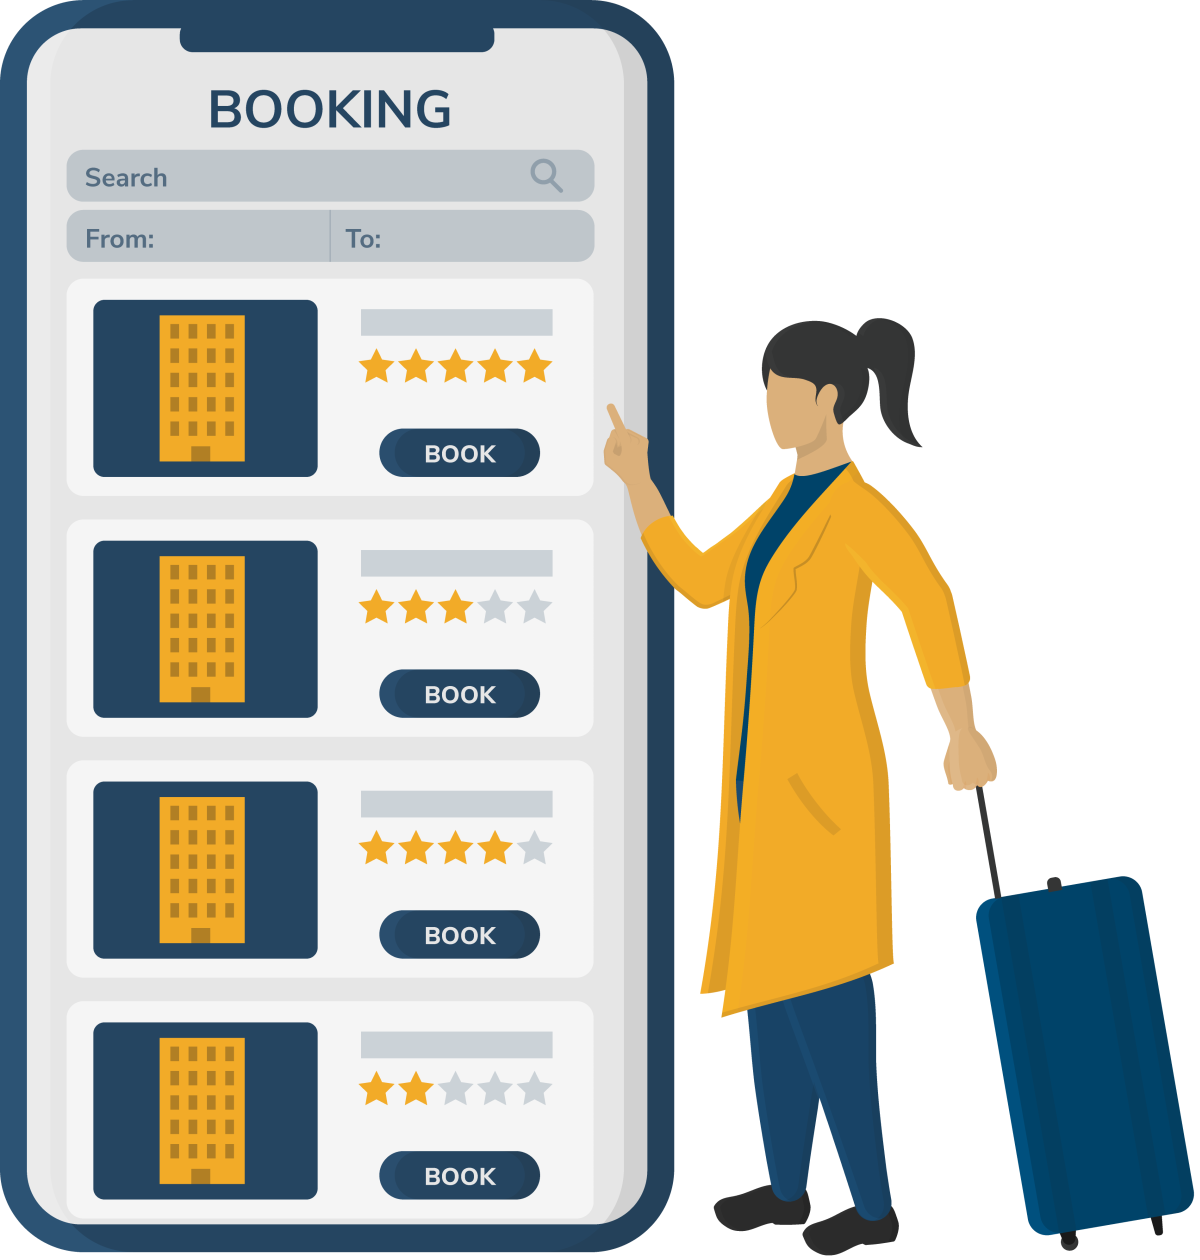
\includegraphics[width=0.15\textwidth]{Images/chapter_18/section_5397940059504640/5281898806116352.png}
 
\end{figure}

\subsection{Expectations from the interviewee}\label{DFpOXaHfjUJHQ4h6AROJx-2}
\\
Numerous components are present in the hotel management system, each with specific constraints and requirements. The following provides an overview of some of the main things the interviewer will want to hear you discuss in more detail.

\subsubsection{Room booking}\label{S57f24fOQm77LOeMGqBoy}
\\
Booking a room is an essential part of the hotel management system. The system must ensure that no two users can book the same room for overlapping time slots. The interviewer expects you to ask questions to identify how the system will work in such situations:

\begin{itemize}
\item
\protect\phantomsection\label{sQKVYkLePfh76XQHz_73n}
How will the system ensure multiple users do not book the same room?
\item
\protect\phantomsection\label{ohIEAiRh0F7Hs0zonxRw0}
What type of users are allowed to book a room in the hotel?
\item
\protect\phantomsection\label{8Q7MD1Ciw4MtLbpSt8gwt}
Can users book a room in advance?
\end{itemize}

\subsubsection{Payment handling}\label{3xcK8PHmI1RSz7-AappTG}
\\
One of the hotel management system's most significant attributes is its payment structure for its customers. This can vary, so the interviewer would expect you to ask the questions listed below:

\begin{itemize}
\item
\protect\phantomsection\label{NzQoecHO5kQE_e-gQVnGr}
What payment methods can the customer use (for example, credit card or cash)?
\item
\protect\phantomsection\label{uQ6WThckIB7HO_s5smMS-}
How is the payment performed? Does the customer pay online or through a receptionist at the hotel?
\item
\protect\phantomsection\label{w0vljN6qBneOQsyALuQVb}
Will the customer be able to pay in advance for a room booking, or is a just-in-time (JIT) payment system available?
\end{itemize}

\subsubsection{Price variance}\label{5U2Z0593L72YgrNeLvwDw}
\\
We touched upon the payment methods of the hotel management system. Now , the pricing model needs to be clarified by the interviewer. Therefore, you may ask the questions listed below:

\begin{itemize}
\item
\protect\phantomsection\label{hjJ5RcjdkG15T_wg89Wju}
How will the booking price be calculated? Or which factors affect the price of a room in the hotel?
\item
\protect\phantomsection\label{tsckLwWLbyI5-eLBt6nrA}
How does the location and size of the room affect its price?
\item
\protect\phantomsection\label{EgyNktkT3a2KQFv6ZWYG0}
How does the booking duration affect the payment?
\end{itemize}

\subsubsection{Booking cancellation}\label{qHzH4gK5pLq_-QEHinXK9}
\\
There will be many duplicate instances in our system. The interviewer expects you to ask the questions provided below:

\begin{itemize}
\item
\protect\phantomsection\label{LJ-is2qBXxwokTq-ExJ12}
Can the user cancel a room booking?
\item
\protect\phantomsection\label{-Qh-g9d6ifeoQnyTHvOy2}
Which type of users are allowed to request a room booking cancellation?
\end{itemize}

\subsection{Design approach}\label{fot8-Doqrg9Zx3EOjlsx2}
\\
We'll design this hotel management system using the bottom-up design approach. For this purpose, we will follow the steps below:

\begin{itemize}
\item
\protect\phantomsection\label{wDS1Vzycoao8ZwoMTMOqL}
Identify and design the smallest components first, such as a room.
\item
\protect\phantomsection\label{GQOk9F9SmajBnOxUiHdZm}
Use these small components to design bigger components, such as building a hotel with multiple rooms.
\item
\protect\phantomsection\label{Vqaob7p7SDGo7oK_Fyi7T}
Repeat the steps above until we design the whole hotel management system.
\end{itemize}

\subsection{Design pattern~}\label{4_xq2OH6NiUOQ-a1zIc3V}
\\
During an interview, discussing the design patterns under which the hotel management system falls is always a good practice. Stating the design patterns gives the interviewer a positive impression and shows that the interviewee is well-versed in the advanced concepts of object-oriented design.
\\
Try to answer the following question. If you are not familiar with design patterns, don't worry! You can learn about them by asking, ``Define design patterns.''

\textbf{Question:}

Which design pattern(s) should be used to design a hotel management system? Please elaborate on your choice(s).

Let's explore the requirements of the hotel management system in the next lesson.

% End of section content